

The source code of TheHive is written mainly in Scala, a general-purpose programming language that runs on the Java Virtual Machine (JVM). The code is organized into several modules and packages, each with a specific purpose and functionality. Figure \ref{fig:modules} shows the structure of the source code.

\begin{figure}[h]
    \centering
    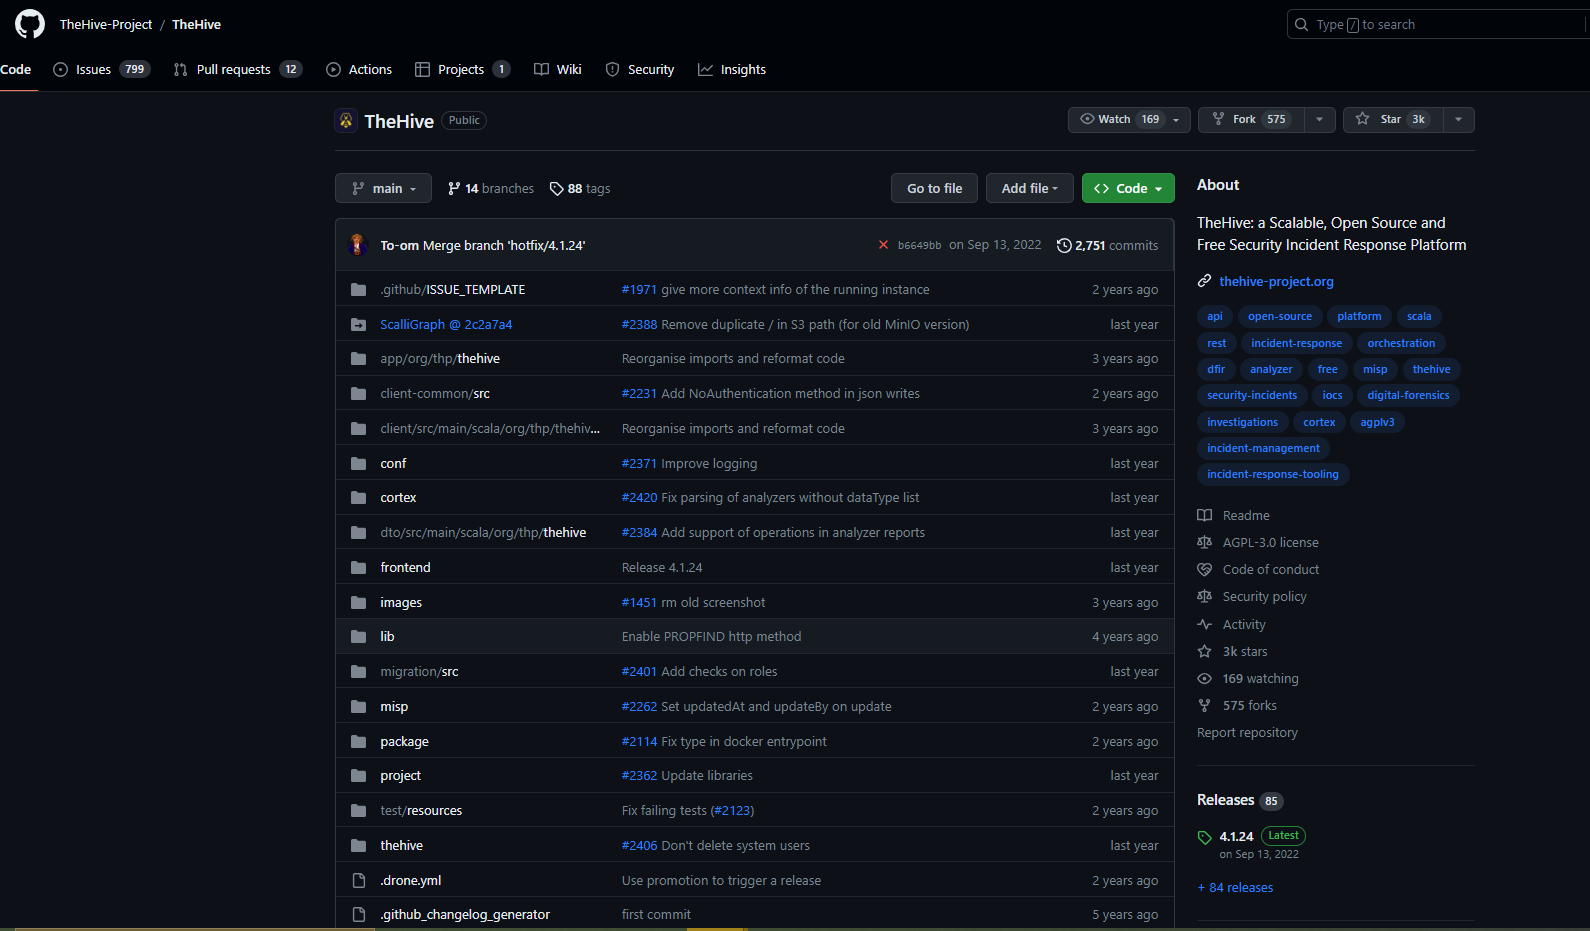
\includegraphics[width=\textwidth]{images/source_code/thehive_src_code.PNG}
    \caption{The structure of the source code of TheHive}
    \label{fig:modules}
\end{figure}

We will briefly describe the main modules and packages of the source code in the following subsections.

\subsection{app}

This module contains the core logic and functionality of TheHive. It includes the following packages:

\begin{itemize}
    \item \texttt{org.thp.thehive}: This package contains the main classes and traits that define the application, such as \texttt{TheHiveApp}, \texttt{TheHiveModule}, and \texttt{TheHiveConfig}.
    \item \texttt{org.thp.thehive.controllers}: This package contains the controllers that handle the HTTP requests and responses for the different endpoints of the application, such as Cases, Tasks, Observables, Alerts, and Users.
    \item \texttt{org.thp.thehive.models}: This package contains the case classes and objects that represent the data models of the application, such as Case, Task, Observable, Alert, User, and Organisation.
    \item \texttt{org.thp.thehive.services}: This package contains the services that provide the business logic and operations for the data models, such as CaseSrv, TaskSrv, ObservableSrv, AlertSrv, UserSrv, and OrganisationSrv.
    \item \texttt{org.thp.thehive.connector}: This package contains the classes and traits that enable the integration with external tools and platforms, such as MISP and Cortex.
\end{itemize}

\subsection{client}

This module contains the code for the web-based user interface of TheHive. It includes the following packages:

\begin{itemize}
    \item \texttt{org.thp.thehive.client}: This package contains the classes and objects that define the client-side application, such as \texttt{ClientApp} and \texttt{ClientConfig}.
    \item \texttt{org.thp.thehive.client.pages}: This package contains the components that render the different pages of the user interface, such as DashboardPage, CasePage, TaskPage, ObservablePage, AlertPage, and UserPage.
    \item \texttt{org.thp.thehive.client.services}: This package contains the services that provide the client-side logic and operations for the user interface, such as ApiService, NotificationService, UserService, and OrganisationService.
\end{itemize}

\subsection{conf}

This module contains the configuration files for the application, such as application.conf and logback.xml.

\subsection{cortex}

This module contains the code for the integration with Cortex. It includes the following packages:

\begin{itemize}
    \item \texttt{org.thp.cortex.client}: This package contains the classes and objects that define the client-side communication with Cortex, such as \texttt{CortexClient} and \texttt{CortexConfig}.
    \item \texttt{org.thp.cortex.dto}: This package contains the case classes and objects that represent the data models of Cortex, such as Analyzer, Job, Report, Responder, Action, Response.
\end{itemize}

\subsection{dto}

This module contains the code for the data transfer objects (DTOs) that are used to exchange data between different layers of the application. It includes the following package:

\begin{itemize}
    \item \texttt{org.thp.thehive.dto}: This package contains the case classes and objects that represent the DTOs of TheHive, such as CaseDTO, TaskDTO, ObservableDTO, AlertDTO, UserDTO.
\end{itemize}

\subsection{frontend}

This module contains the code for building and packaging the frontend assets of TheHive. It includes files such as webpack.config.js and package.json.

\subsection{lib}

This module contains some third-party libraries that are used by TheHive. It includes files such as scalagraph.jar and elastic4play.jar.

\subsection{migration}

This module contains some scripts and tools for migrating data from previous versions of TheHive. It includes files such as migration.sh and migration.conf.

\subsection{misp}

This module contains some scripts and tools for synchronizing data with MISP. It includes files such as misp.sh and misp.conf.

\subsection{project}

This module contains some files for managing the project dependencies and build process. It includes files such as build.sbt and plugins.sbt.

\subsection{test}

This module contains some files for testing the application. It includes files such as test.conf and test.sh.

% \section{Conclusion}

% TheHive is a powerful and user-friendly security incident response platform that is developed by a passionate community of security experts and enthusiasts. The source code of TheHive is open source and free, and anyone can access, review, or contribute to it on GitHub. The source code is written mainly in Scala, and is organized into several modules and packages, each with a specific purpose and functionality. We have provided a high level overview of the main modules and packages of the source code, and explained their purpose and functionality.


